\documentclass[11pt]{ctexart}

\usepackage[S]{dryNote}
\usepackage{dryNotation}
\usepackage{tabularx}
\usepackage[toc]{multitoc}
\usepackage{gbt7714}

\title{概率论与数理统计习题课-1\textsuperscript{st}}
\author{其实只是一份复习提纲}
\date{2024 年 10 月 20 日}

\begin{document}
\maketitle
{ 	
	\footnotesize
	\keben
	\tableofcontents
}

\addtocontents{toc}{\protect\setcounter{tocdepth}{2}}
%%%%%%%%%%%%%%%%%%%%%%%%%%%%%%%%%%%%%%%%%%%%%%%%%%%%%%%%%%%%%%%%%%%%%%%%
\section{概率论的方法论}

\begin{table}[H]
	\centering
\begin{tabular}{ccccc}
	\toprule
		(随机试验产生的)事件 & $\Longleftrightarrow$ & (样本空间的)集合 & $\longrightarrow$ & 概率 \\
	\midrule
		事件描述 & $\Longleftrightarrow$ & 集合运算 & $\longrightarrow$ & 概率运算 \\
	\bottomrule
\end{tabular}
\end{table}

具体地说, 事件$A$ 、$B$同时发生对应交集$A \cap B$, $A$或$B$发生对应并集$A \cup B$, $A$不发生对应余集$\bar A$, $A$发生但$B$不发生对应差集$A - B$. 
再对集合赋予概率, 就可以开心地计算形形色色事件的概率啦. 
回忆概率的定义\cite{shengzhou:2020a}: 
\begin{definition}[概率]\label{def:prob}
	设$E$是随机试验, $S$是它的样本空间. 
	对于$E$的每一个事件$A$赋予一个实数, 记为$\P(A)$, 称为事件$A$的\emph{概率}, 如果集合函数$\P(\cdot)$满足下列条件: 
	\begin{enumerate}[label=(\arabic*)]
		\item {\keben 非负性:} 对每一个事件$A$, 有$\P(A) \geq 0$. 
		\item {\keben 规范性:} 对于必然事件$S$, 有$\P(S) = 1$. 
		\item {\keben 可列可加性:} 设$A_1, A_2, \dots$是两两互不相容的事件, 则有
			\begin{equation*}
				\P(A_1 \cup A_2 \cup \dots) = \P(A_1) + \P(A_2) + \dots. 
			\end{equation*}
	\end{enumerate}
\end{definition}

在定义的基础上, 不难证明概率有如下性质. 
\begin{enumerate}[label=(\arabic*)]
	\item $\P(\varnothing) = 0$. 
	\item {\keben 有限可加性}. 
	\item 若$A \subset B$, 则$\P(B - A) = \P(B) - \P(A) \geq 0$, 从而$\P(B) \geq \P(A)$.  
	\item 事件的概率总不超过$1$. 
	\item {\keben 逆事件的概率} $\P(\bar A) = 1 - \P(A)$. 
	\item {\keben 加法公式} $\P(A \cup B) = \P(A) + \P(B) - \P(A \cap B)$.
\end{enumerate}
\begin{proof}
	\begin{enumerate}[label=(\arabic*)]
		\item 对任意集合$A$, 由$\P(A) = \P(A \cup \varnothing) = \P(A) + \P(\varnothing)$可得. 
		\item 在可列可加性中, 取$A_k = \varnothing$, $k > n$即可. 
		\item 注意到$A \cap (B - A) = \varnothing$, $A \cup (B - A) = A \cup B = B$, 由有限可加性可得.
		\item 任何事件$A$都是$S$的子集, 由上一性质有$\P(A) \leq \P(S) = 1$. 
		\item 由有限可加性可得. 
		\item  由性质(3), $\P(A \cup B) - \P(A) = \P(A \cup B - A) = \P(B) - \P(A \cap B)$. 
	\end{enumerate}
\end{proof}

\begin{remark}
	逆事件概率在做题中常常有简化计算的作用, 关键词通常为“至少”. 
\end{remark}

%%%%%%%%%%%%%%%%%%%%%%%%%%%%%%%%%%%%%%%%%%%%%%%%%%%%%%%%%%%%%%%%%%%%%%%%
\section{条件概率、独立性}

\subsection{基础知识}

有的时候, 我们要考察在给定某些事件下另一些事件发生的概率. 
这个时候需要利用已知的信息之间的关系去搭建桥梁, 进而解决概率问题. 
例如, 在事件$B$发生的情况下, 事件$A$发生的概率.
此时我们考虑的样本空间应该是$B$——作为先决条件, 在此基础上, 对$A$发生的概率进行重整化
\begin{equation*}
	\P(A | B) = \frac{\P(A \cap B)}{\P(B)}, 
\end{equation*}
称作事件$A$在事件$B$发生下的\emph{条件概率}.
事实上, 一切概率都可以看作条件概率: 在定义\ref{def:prob}的记号下, 
\begin{equation*}
	\P(A | S) = \frac{\P(A \cap S)}{\P(S)} = \frac{\P(A)}{1}. 
\end{equation*}
于是条件概率$\P(\cdot | A)$也满足概率的诸多性质. 
在此基础上, 我们有三个重要公式: 
\begin{itemize}
	\item {\keben 乘法公式} $\P(A \cap B) = \P(B | A) \P(A)$. 
	\item {\keben 全概率公式} 称$B_1, \dots, B_n$为$S$的一个划分, 如果$B_1 \cup B_2 \cup \dots \cup B_n = S$且$B_i \cap B_j = \varnothing$, $\forall i, j$. 若$B_i > 0$, $\forall i$, 则
		\begin{equation*}
			\P(A) 
			= \sum_{i=1}^n \P(A \cap B_i)
			= \sum_{i=1}^n \P(B_i) \P(A | B_i). 
		\end{equation*}
	\item {\keben 贝叶斯公式} 设$B_1, \dots, B_n$为$S$的一个划分, 且$\P(B_i) > 0$, $\forall i$,  $\P(A) > 0$, 则
		\begin{equation*}
			\P(B_i | A)
			= \frac{\P(A \cap B_i)}{\P(A)}
			= \frac{\P(B_i) \P(A | B_i)}{\sum_{i=1}^n \P(B_i) \P(A | B_i)}. 
		\end{equation*}
\end{itemize}

\begin{remark}
	从形式上看, 贝叶斯公式不过是条件概率定义与全概率公式的简单推论, 为什么它很重要?  
	辩证唯物主义告诉我们, 在一个具体的因果联系中, 原因在前, 结果在后, 二者不能混淆和颠倒. 
	然而在现实生活中, 我们常常需要执“果”索“因”: 对于事件的结果分析可能原因. 
	贝叶斯公式就给了我们这种能力. 
%	
%	例如我们把事件$A$看作结果, 事件$B_1, \dots, B_n$看作导致这一结果所有可能的原因. 
%	$\P(B_i)$是在没有进一步信息(不知道$A$发生)的情况下, 人们对事件$B_i$发生可能性大小的认识. 
%	$\P(B_i | A)$则是在有了新信息(知道$A$发生)后, 人们对事件$B_i$发生可能性大小的新认识. 
%	且看示例\ref{ex:Bayes-CancerTest}. 
\end{remark}

特别地, 当$\P(A B) = \P(A) \cdot \P(B)$时, 我们称事件$A$和事件$B$\emph{独立}. 
此时有$\P(B | A) = \P(B)$, $\P(A | B) = \P(A)$, 意味着事件$A$(或$B$)的发生对事件$B$(或$A$)没有影响. 
除非明确给出相互独立的条件, 我们通常需要计算概率来验证两者是否独立. 


\subsection{例题}

\begin{example}
某产品的合格品率为$99\%$. 
已知一个合格产品使用10年以上的概率达到$0.9$, 而一个不合格产品使用10年以上的概率仅为$0.6$.
求: 
\begin{enumerate}
	\item 任取一个该产品, 它能使用10年以上的概率;
	\item 已知一个产品已经使用了10年还能正常工作的条件下, 它是合格品的概率. 
\end{enumerate}
\end{example}
\begin{solution}
	设$A$表示产品为合格品, $B$表示产品正常使用10年以上. 
	于是$\P(A) = 0.99$, $\P(B | A) = 0.9$, $\P(\bar B | \bar A) = 0.6$. 
	\begin{enumerate}
		\item $\P(B) = \P(B \cap A) + \P(B \cap \bar A) = \P(A) \cdot \P(B | A) + \P(\bar A) \cdot \P(B | \bar A)$. 
		\item 本题需要我们利用贝叶斯公式计算$\P(A|B)$: 
			\begin{equation*}
				\P(A|B)
				= \frac{\P(A \cap B)}{\P(B)}
				= \frac{ \P(A) \cdot \P(B | A)}{\P(A) \cdot \P(B | A) + \P(\bar A) \cdot \P(B | \bar A)}. 
			\end{equation*}
	\end{enumerate}
\end{solution}

\begin{example}[贝叶斯公式的应用]\label{ex:Bayes-CancerTest}
	一种诊断某种癌症的试剂, 经临床试验有如下记录: 癌症患者试验的结果是阳性的概率是$95 \%$, 非癌症患者试验的结果是阴性的概率是$95 \%$. 
	现用这种试剂在某社区进行癌症普查, 设该社区发病率为$0.5 \%$, 问某人反应为阳性时, 该如何判断他是否患有癌症?\cite{weilaisheng:2024a} 
\end{example}
\begin{solution}
	设$A$表示“测试阳性”的事件, 是结果, $B$表示“患癌症”的事件, 是原因. 
	于是题目条件可以翻译为$\P(A | B) = 0.95$, $\P(\bar A | \bar B) = 0.95$, $\P(B) = 0.005$.
	现在要计算的是他是否患癌的概率, 由贝叶斯公式, 
	\begin{align*}
		\P(B | A)
		&= \frac{\P(A \cap B)}{\P(A)}
		= \frac{\P(B) \P(A | B)}{\P(B) \P(A | B) + \P(\bar B) \P(A | \bar B)} \\
		&= \frac{0.005 \times 0.95}{0.005 \times 0.95 + (1-0.005) \times (1-0.95)}
		= 8.7 \%
	\end{align*}
	事实上, 这个人患癌的概率的可能性很小, 可以告诉他不必紧张, 可以去做进一步的检查. 	
\end{solution}


%%%%%%%%%%%%%%%%%%%%%%%%%%%%%%%%%%%%%%%%%%%%%%%%%%%%%%%%%%%%%%%%%%%%%%%%
\section{一维随机变量及其分布}

我们把“用来表示随机现象结果的变量”称作“随机变量”. 
更为数学化的定义是, 随机变量$X$是样本空间$S$上的实值函数. 
我们常用大写字母$X, Y, Z$来表示随机变量, 小写字母$x, y , z$来表示它的取值. 
\begin{itemize}
	\item 如果随机变量的可能取值是有限个或者可列无限个, 则称{\keben 离散型随机变量},
	\item 如果随机变量的可能取值范围充满了数轴的某一个区间$(a, b)$, 则称{\keben 连续型随机变量}, 这里的$a$可以是$- \infty$, $b$可以是$+ \infty$. 
\end{itemize}

\subsection{一维离散型随机变量及其分布}
 
我们习惯用{\keben 分布律}来描述离散型随机变量: 离散型随机变量$X$的所有可能取值为$x_k$, $k = 1, 2, \dots$, 它的分布律为
\begin{equation*}
	\P \{ X = x_k \} = p_k, \quad k =1,2,\dots. 
\end{equation*} 
由于分布律的取值依然是概率, 它自然地继承了概率的如下性质: 
\begin{enumerate}[label=(\arabic*)]
	\item {\keben 非负性:} $p_k \geq 0$, $k = 1, 2, \dots$. 
	\item {\keben 规范性:} $\sum_k p_k = 1$. 
\end{enumerate}

\subsubsection{$0-1$分布/两点分布/伯努利分布}

虽然给出了三个名字, 但是都是在说同一件事情——{\keben 一重伯努利试验}. 
伯努利试验是只有两种结果(即两点)的试验, 不妨记为事件(集合)$A$及其对立面$\bar A$, 它的分布律为$\P(A) = p$, $\P(B) = 1 - p$, 其中$p \in [0,1]$. 

如果我们把事件$A$和$\{X = 1\}$, 事件$\bar A$和$\{ X = 0\}$对应起来, 得到取值为$0-1$的随机变量$X$. 
其分布律为
\begin{table}[H]
	\centering
\begin{tabular}{c|c c}
	\toprule
		X & $0$ & $1$ \\
	\midrule
		$p_k$ & $1-p$ & $p$ \\
	\bottomrule
\end{tabular}
\end{table}
\noindent
称这样的随机变量$X$服从参数为$p$的$0-1$分布, 记做$X \sim B(1, p)$. 


\subsubsection{二项分布}

进一步地, 我们把伯努利试验{\keben 独立地重复进行$n$次}, 称为$n$重伯努利试验. 
用$X$表示结果$A$出现的次数, 则其分布律为
\begin{equation*}
	\P \{ X = k \} = C_n^k p^k (1-p)^{n-k}, \quad k = 1,2, \dots,  
\end{equation*}
称$X$服从参数为$n, p$的二项分布, 记做$X \sim B(n, p)$. 

当然, $n=1$时我们进行的是一重伯努利试验, 此时分布退化为$0-1$分布. 

\begin{remark}
	在具体应用中, 我们可能很少会看见“随机变量$X$服从参数为$n, p$的二项分布”之类的表述——更多的是要求我们把关心的事件记为$A$, 关心的事件的对立面记为$\bar A$——尽管结果可能不止一种, 但我们要一分为二地看待问题. 
	例如经典的摸小球试验中, 可能有很多种小球, 我们关心的事情是“摸到了红球”与“没有摸到红球”. 
\end{remark}

\subsubsection{几何分布}

很多时候我们关心这样的问题: 摸到红球的概率为$p$, 第$k$次才摸到红球的概率; 或者试验成功的概率为$p$, 第$k$次才成功的概率. 

即在多重伯努利试验中, 我们关心的事件发生的概率为$p$, $X$表示我们关心的事件首次发生时进行的试验次数, 那么$X = k$意味着前$k-1$次我们关心的事件并未发生, 第$k$次才发生, 于是
\begin{equation*}
	\P \{ X = k \} = (1-p)^{k-1} p. 
\end{equation*}
我们称这样的$X$满足参数为$p$的几何分布.
这样的分布律具有几何级数的形式: 当$p \in (0,1)$时
\begin{equation*}
	\sum_{k=1}^{\infty} \P\{ X = k \}
	= p \sum_{k=1}^{\infty} (1-p)^{k-1} 
	= p \cdot \frac{1}{1 - (1-p)}
	= 1. 
\end{equation*}

\subsubsection{超几何分布}
超几何分布是描述在“有限个对象中(无放回地、等可能地)抽出$n$个对象, 成功抽出$k$次指定种类的对象”的分布. 

例如袋中有$r$个红球和$b$个黑球, 现从中无放回地摸出$n$个球, 随机变量$X$表示摸出的红球的个数, 则当$0 \leq n \leq \min\{r, b\}$时, 摸出$k$个红球意味着同时摸出了$n-k$个黑球, 于是
\begin{equation*}
	\P \{X=k\} = \frac{C_r^k C_b^{n-k}}{C_{r+b}^n}. 
\end{equation*}

\subsubsection{泊松分布}

若随机变量$X$的分布律为
\begin{equation*}
	\P \{X = k\} = \frac{\lambda^k e^{-\lambda}}{k !}, 
\end{equation*}
其中常数$\lambda > 0$, 则称$X$服从参数为$\lambda$的泊松分布, 记做$X \sim \pi(\lambda)$. 

%\vspace{.3cm}
\noindent\textbf{\large\keben 泊松定理}

泊松定理告诉我们, 在一定程度上二项分布可以被的泊松分布近似. 


\begin{theorem}[泊松极限定理]
	设$\{p_n\}_{n=1}^\infty$为$[0,1]$中的实数列, 如果$n p_n \to \lambda$, 那么有
	\begin{equation*}
		\lim_{n \to \infty} C_n^k p_n^k (1-p_n)^{n-k} = \frac{\lambda^k e^{-\lambda}}{k !}. 
	\end{equation*}
\end{theorem}

于是当$X \sim B(n,p)$中$n$较大、$p$较小时, 我们引入随机变量$Y \sim \pi(np)$, 可以对二项分布的分布律做如下近似计算: 
\begin{equation*}
	\P(X = k) = C_n^k p^k (1-p)^{n-k} \approx \frac{(np)^k e^{-np}}{k!} = \P(Y = k)
\end{equation*}

背景: 单位时间(或单位面积、单位产品等)上某稀有事件(这里稀有事件是指不经常发生的事件)发生的次数常服从泊松分布$\pi(\lambda)$, 其中$\lambda$为该稀有事件发生的强度. 

\subsubsection{例题}

对于抽样问题, 我们按下述方法确定概率模型: 
\begin{equation*}
	\begin{cases}
		\textbf{一次取样: } \quad \text{$0-1$分布} \\
		\textbf{多次取样} 
			\begin{cases}
				\textbf{无放回: } &\text{超几何分布 } \\
				\textbf{有放回: } &\text{二项分布 }
			\end{cases}
	\end{cases}
\end{equation*}
而“第几次才有如何如何的结果”考察的是几何分布. 

\begin{example}[二项分布] 
	经验表明:预订餐厅座位而不来就餐的顾客比例为$20\%$. 
	如今餐厅有50个座位, 但预订给了52位顾客, 问到时顾客来到餐厅而没有座位的概率是多少?
\end{example}
\begin{solution}
	记$X$为预订的52位顾客中不来就餐的顾客数, 则$X \sim B(52, 0.2)$
	因为“顾客来到餐厅没有座位”相当于“52位顾客中最多1位顾客不来就餐”, 所以所求概率为
	\begin{equation*}
		\P\{X \leq 1\}
		= \P\{X = 0\} + \P\{X = 1\}
		= 0.8^{52} + 52 \times 0.8^{51} \times 0.2
		=0.000 127 9.
	\end{equation*}
\end{solution}

\begin{example}[泊松定理的应用]
	一批产品的不合格品率为0.02. 
	现从中任取40件进行检查, 若发现两件或两件以上不合格品就拒收这批产品. 
	分别用以下方法求拒收的概率:
	\begin{enumerate}
		\item 用二项分布作精确计算; 
		\item 用泊松分布作近似计算. 
	\end{enumerate}
\end{example}
\begin{solution}
	解记$X$为抽取的40件产品中的不合格品数, 则$X \sim B(40, 0.02)$, 而“拒收”就相当于$\{X>2\}$. 
	\begin{enumerate}
		\item 拒收的概率为
			\begin{align*}
				\P\{X \geq 2\} 
				&= 1 - \P\{X = 0\} - \P\{X = 1\} \\
				&= 1 - 0.98^{40} - 40 \times 0.98^{39} \times 0.02
				= 0.1905. 
			\end{align*}
		\item 设$Y \sim \pi(40 \times 0.02) = \pi(0.8)$, 用泊松分布作近似计算, 可得近似值为
			\begin{align*}
				\P\{X \geq 2\}
				&= 1 - \P\{Y = 0\} - \P\{Y = 1\} \\
				&= 1 - e^{-0.8} - 0.8 \times e^{-0.8}
				= 0.1912. 
			\end{align*}
	\end{enumerate}
	可见近似值与精确值相差$0.0007$, 近似效果较好. 
\end{solution}


\subsection{一维连续型随机变量及其分布}

对于某个子集$I \subseteq \R$, 事件$\{X \in I\}$相当于$\{s \in S \colon X(s) \in I\}$, 于是它的概率$\P\{X \in I\}$实际上是$\P\{s \in S \colon X(s) \in I\}$. 
特别地, 我们关心形如$(- \infty, t]$的区间, 称
\begin{equation*}
	F_X(t) := \P(X \in (-\infty, t]) = \P(X \leq t), \quad t \in \R
\end{equation*}
为$X$的{\keben 分布函数}. 
当我们讨论的随机变量没有歧义的时候, 我们可以略去$X$, 简记为$F(t)$.
分布函数有如下性质: 
\begin{enumerate}[label=(\arabic*)]
	\item {\keben 单调性:} $F(x)$是非减函数; 
	\item {\keben 有界性:} $F(-\infty) = \lim_{x \to -\infty}F(x) = 0$, $F(+\infty) = \lim_{x \to +\infty}F(x) = 1$. 
	\item {\keben 右连续性:} $\lim_{x \downarrow x_0}F(x) = F(x)$.\footnote{证明思路大致是: 对任意$x_n \downarrow x$, $0 \leq F(x_n) - F(x) = \P(x < X \leq x_n) \to \P(\varnothing) = 0$. }
\end{enumerate}
反之, $\R$上任何一个具备以上三条性质实值函数, 一定是某个随机变量的分布函数, 即以上三条性质是分布函数的根本性质. 

可以用分布函数$F(t)$来表示下列概率: 
\begin{enumerate}[label=(\arabic*)]
	\item $\P(X \leqslant a)=F(a)$;
	\item $\P(X<a)=F(a-0)$;
	\item $\P(X>a)=1-\P(X \leqslant a)=1-F(a)$;
	\item $\P(X=a)=\P(X \leqslant a)-\P(X<a)=F(a)-F(a-0)$;
	\item $\P(X \geqslant a)=1-\P(X<a)=1-F(a-0)$;
	\item $\P(a < X \leq b) = \P(X \leq b) - \P(X \leq a) = F(b) - F(a)$; 
	\item $\P(|X|<a)=\P(X<a)-\P(X \leqslant-a)=F(a-0)-F(-a)$. 
\end{enumerate}


分布函数可以用于描述任意类型的随机变量: 
离散型随机变量的分布函数是右连续的阶梯函数.
\begin{figure}[H]
	\centering
	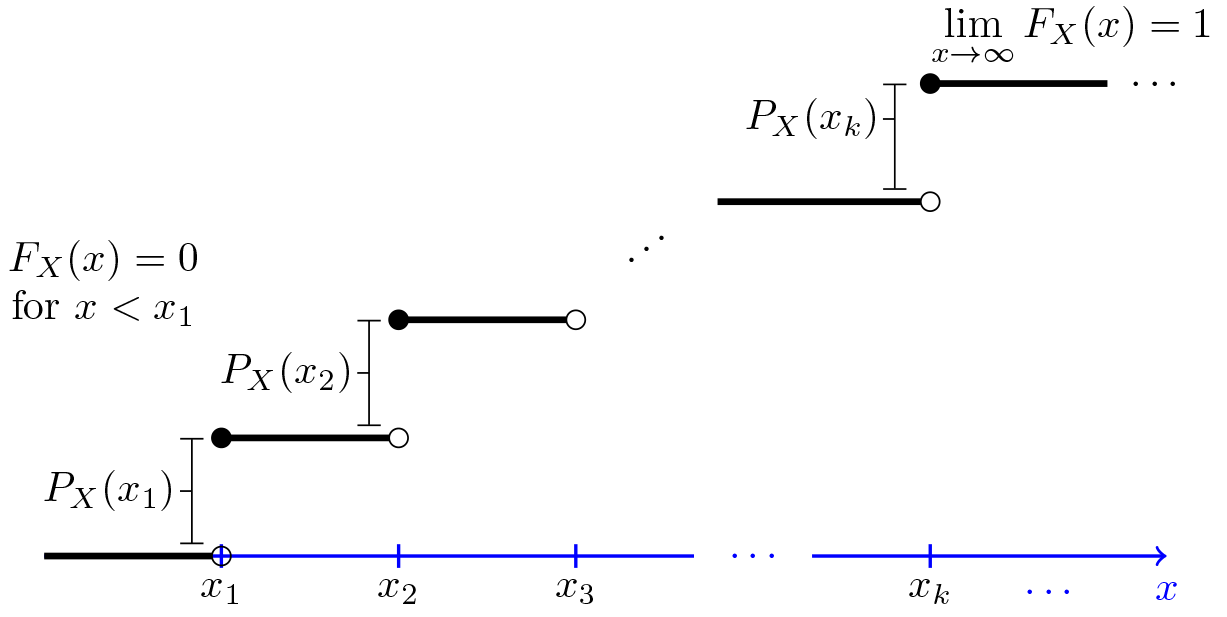
\includegraphics[width = .7 \textwidth]{figure/CDF-Discrete_b.png}
\end{figure}
\noindent
连续型随机变量的分布函数既是右连续的, 也是左连续的, 进一步地, 在任一点的取值的概率为$\P\{X = x\} = F(x) - F(x - 0) = 0$. 

对于连续型随机变量$X$的分布函数$F(x)$, 若存在非负函数$f(x)$使得对任意实数$x$, 使得
\begin{equation*}
	F(x) = \int_{\infty}^x f(t) \dd t, \quad \forall x \in \R, 
\end{equation*}
那么称$f(x)$为$X$的{\keben 概率密度函数}. 
于是连续型随机变量$X$在某一区间的概率为
\begin{align*}
	&\P\{a \leq X \leq b\}
	= \P\{a \leq X < b\}
	= \P\{a < X < b\}
	=\P\{a < X \leq b\} \\
	=& F(b) - F(a)
	= \int_a^b f(x) \dd x. 
\end{align*}
概率密度函数具有如下性质: 
\begin{enumerate}[label=(\arabic*)]
	\item {\keben 非负性:} $f(x) \geq 0$; 
	\item {\keben 正则性:} $\int_{-\infty}^{+\infty} f(x) \dd x = 1$. 
\end{enumerate}
反之, $\R$上任何一个具备以上两条性质实值函数$g(x)$, 一定是某个随机变量的概率密度函数, $G(x):= \int_{-\infty}^x g(t) \dd t$是这个随机变量的分布函数. 
换而言之, 以上两条性质是概率函数的根本性质. 

\begin{theorem}
	若概率密度函数$f$在$x$处连续, 那么$F'(x) = f(x)$	
\end{theorem}


\subsubsection{均匀分布}
若随机变量$X$的概率密度函数为
\begin{equation*}
	f(x) = 
	\begin{cases}
		\frac{1}{b-a}, & a < x < b, \\
		0, &\text{其它},
	\end{cases}
\end{equation*}
则称$X$服从区间$(a, b)$上的均匀分布, 记做$X \sim U(a, b)$. 

背景: 向区间$(a, b)$随机投点, 落点坐标$X$一定服从均匀分布$U(a, b)$. 
这里 “随机投点”是指: 点落在任意相等长度的小区间上的可能性是相等的. 

\subsubsection{正态分布}

若随机变量$X$的概率密度函数为
\begin{equation*}
	f(x) = \frac{1}{\sqrt{2 \pi} \sigma} e^{- \frac{(x-\mu)^2}{2 \sigma^2}}
\end{equation*}
其中标准差$\sigma > 0$, 均值$\mu$为常数, 则称$X$服从参数为$\mu, \sigma$的正态分布, 记做$X \sim N(\mu, \sigma)$. 
概率密度函数$f(x)$形如钟形曲线, 关于$\mu$对称且在$\mu$处取得最大值, 于是
\begin{equation*}
	\P\{X \geq \mu + t\} = \P\{X \leq \mu - t\} = F_X(\mu - t). 
\end{equation*}
\begin{itemize}
	\item 固定$\sigma$, 改变$\mu$的值: 这相当于我们改变了对称轴$x = \mu$, 函数形状不发生改变, 整体左右移动. 
	\item 固定$\mu$, 改变$\sigma$的值: 函数对称轴不变, $\sigma$越大, 图形越平坦, 落在$\mu$附近的概率减小; $\sigma$越小, 图形越陡峭, 落在$\mu$附近的概率增大. 或者说, $\sigma$控制了分布的分散程度. 
\end{itemize}
特别地, 称分布$N(0, 1)$为{\keben 标准正态分布}, 其概率密度函数的形式较为简单: 
\begin{equation*}
	\varphi(x) = \frac{1}{\sqrt{2 \pi}} e^{- \frac{x^2}{2}}. 
\end{equation*}


正态分布的分布函数
\begin{equation*}
	F(x) = \frac{1}{\sqrt{2 \pi} \sigma} \int_{- \infty}^{x} e^{- \frac{(t-\mu)^2}{2 \sigma^2}} \dd t
\end{equation*}
是难以计算的. 
对于$X \sim N(\mu, \sigma)$, 通常我们会对它做线性变换{\keben 标准化}、再查阅标准正态分布表来得到$X$在某一区间的概率——$Z = (X - \mu) / \sigma$服从标准正态分布: 
\begin{align*}
	\P\{Z \leq x\}
	&= \P\{ X \leq \mu + \sigma x\}
	= \frac{1}{\sqrt{2 \pi} \sigma} \int_{- \infty}^{\mu + \sigma x} e^{- \frac{(t-\mu)^2}{2 \sigma^2}} \dd t \\
	&= \frac{1}{\sqrt{2 \pi}} \int_{- \infty}^{x} e^{- \frac{s^2}{2}} \dd s
	=: \Phi(x), 
\end{align*}
其中$\Phi(x)$为标准正态分布的分布函数. 
于是
\begin{equation*}
	\P(a < X \leq b)
	= \P\left(\frac{a - \mu}{\sigma} < Z \leq \frac{b - \mu}{\sigma} \right)
	= \Phi\left(\frac{b - \mu}{\sigma} \right) - \Phi\left(\frac{a - \mu}{\sigma}\right). 
\end{equation*}
当$t \geq 0$时, $\Phi(t)$可以直接查表得出; 而当$t < 0$时, 利用$\varphi(x)$关于$x = 0$对称可得
\begin{equation*}
	\Phi(t) 
	= \int_{-\infty}^t \varphi(x) \dd x 
	= \int_{-t}^{+\infty} \varphi(x) \dd x 
	= 1 - \Phi(-t). 
\end{equation*}

此外, 正态分布“几乎所有”的值都在平均值正负三个标准差的范围内, 这被称为{\keben $3\sigma$原则}. 
\begin{figure}[H]
	\centering
	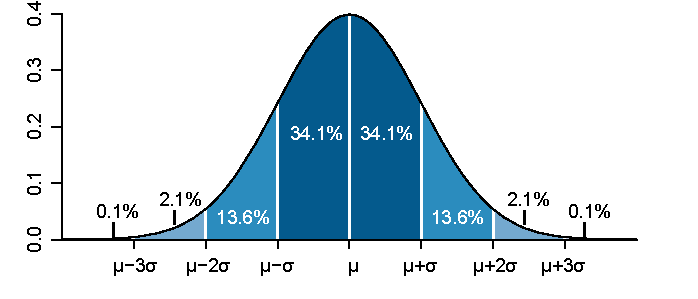
\includegraphics[width = .7 \textwidth]{figure/Standard_deviation_diagram_micro.pdf}
\end{figure}

背景: 一个变量若是由大量微小的、独立的随机因素的叠加结果, 则此变量一般是服从正态分布的. 
测量误差就是由量具偏差、测量环境的影响、测量技术的影响、测量人员的心理影响等随机因素叠加而成的, 所以通常认为测量误差常服从正态分布. 

\subsubsection{指数分布}

若随机变量$X$的概率密度函数为
\begin{equation*}
	f(x) = 
		\begin{cases}
			\lambda e^{-\lambda x}, & x > 0, \\
			0, & x\leq 0, 
		\end{cases}
\end{equation*}
其中参数$\lambda > 0$, 则称$X$服从参数为$\lambda$的指数分布, 记做$X \sim Exp(\lambda)$. 
其分布函数为
\begin{equation*}
	F(x) = 
		\begin{cases}
			1 - e^{\lambda x}, & x > 0, \\
			0, & x \leq 0. 
		\end{cases}
\end{equation*}

指数分布具有{\keben 无记忆性}: 
\begin{equation*}
	\P\{ X > s + t | X > s\}
	= \frac{\P\{ X > s+t \}}{\P\{ X > s \}}
	= \frac{1 - F(s+t)}{1 - F(s)} 
	= 1 - F(t)
	= \P\{X > t\}. 
\end{equation*}

背景: 若一个元器件(或一台设备, 或一个系统)遇到外来冲击时即告失效, 则首次冲击来到的时间$X$(寿命)服从指数分布. 
很多产品的寿命可认为服从或近似服从指数分布. 

\subsubsection{例题}

\begin{example}[概率密度函数]
	设$f(x)$, $g(x)$都是概率密度函数, 求证: 
	\begin{equation*}
		h(x) = \alpha f(x) + (1-\alpha) g(x), \quad 0 \leq \alpha \leq 1
	\end{equation*}
	也是概率密度函数, 
\end{example}
\begin{proof}
	只需验证$h(x)$满足非负性与正则性即可: 由于$\alpha f(x) \geq 0$, $(1-\alpha) g(x) \geq 0$, 从而$h(x) \geq 0$, 此外
	\begin{equation*}
		\int_{-\infty}^{+\infty} h(x) \dd x
		= \alpha \int_{-\infty}^{+\infty}  f(x) \dd x + (1-\alpha) \int_{-\infty}^{+\infty}  g(x) \dd x
		= \alpha + (1-\alpha)
		= 1. 
	\end{equation*}
\end{proof}

\begin{example}[均匀分布]
	设$K$服从$(1, 6)$上的均匀分布, 求方程$x^2 + K x + 1 = 0$有实根的概率. 
\end{example}
\begin{solution}
	方程$x^2 + K x + 1 = 0$有实根的充要条件是
	\begin{equation*}
		\{K^2 - 4 \geq 0\} = \{K \leq -2\} \cup \{K \geq 2\}.  
	\end{equation*}
	而$K \sim U(1,6)$, 因此所求概率为
	\begin{equation*}
		\P\{K \leq 2\} + \P\{K \geq 2\}
		= 0 + \int_2^6 \frac{1}{5} \dd x 
		= 0.75
	\end{equation*}
\end{solution}

\begin{example}[正态分布]
	设随机变量$X$服从正态分布$N(\mu, \sigma)$, 试问: 随着$\sigma$的增大, 概率$\P(|X-\mu|<\sigma)$是如何变化的?
\end{example}
\begin{proof}
	\begin{equation*}
		\P\{|X - \mu| < \sigma\}
		= \P\left\{ -1 < \frac{X - \mu}{\sigma} < 1 \right\}
		= \Phi(1) - \Phi(-1)
		\approx 0.6826. 
	\end{equation*}
	于是概率$\P(|X-\mu|<\sigma)$与$\sigma$无关. 这也是$3\sigma$原则的来源. 
\end{proof}

\begin{example}[指数分布、二项分布]
	设顾客在某银行的窗口等待服务的时间$X$(以分钟计)服从指数分布, 其密度函数为
	\begin{equation*}
		f(x) = 
			\begin{cases}
				\frac{1}{5} e^{-\frac{x}{5}}, & x > 0, \\
				0, & x \leq 0. 
			\end{cases}
	\end{equation*}
	某顾客在窗口等待服务, 若超过10分钟他就离开. 
	他一年要到银行5次, 以$Y$表示一年内他未等到服务而离开窗口的次数, 试求$\P(Y \geq 1)$. 
\end{example}
\begin{solution}
	$Y \sim B(5, p)$, 其中$p = \P\{X > 10\} = \int_{10}^{+\infty} \frac{1}{5} e^{-\frac{x}{5}} \dd x = e^{-2}$, 所以得
	\begin{equation*}
		\P(Y \geq 1)
		=1-\P(Y=0)
		=1-(1-p)^{5}
		=1-(1-e^{-2})^5
		\approx 0.516 7.
	\end{equation*}
\end{solution}

\subsection{随机变量函数的分布}


若$X$为离散型随机变量, 那么它的函数$Y = g(X)$也一定是离散型随机变量. 
设$X$的可能取值集合为$\{x_k\}$, 那么$Y$的可能取值集合为$\{g(x_k)\}$. 
如果其中有某些值相等, 则把那些相等的值分别合并, 并把对应的概率相加即可得到$Y$的分布律. 

若连续型随机变量$X$的概率密度函数为$f_X(x)$, 考虑随机变量$Y = g(X)$, 我们先求出$Y$的分布函数
\begin{equation*}
	F_Y(y) = \P\{g(X) \leq y\}, 
\end{equation*}
再通过求导得出$Y$密度函数. 
特别地, 当$g(x)$严格单调, 其反函数$h(y)$导函数连续时, 
\begin{equation}\label{eq:DensityofFun}
	f_Y(y) = 
	\begin{cases}
		f_X(h(y)) \cdot |h'(y)|, & a < y < b, \\
		0, &\text{其他}. 
	\end{cases}
\end{equation}

\subsubsection{例题}

\begin{example}
	设$X \sim U(0,1)$. 
	\begin{enumerate}
		\item 求$Y = e^X$的概率分布. 
		\item 求$Y = -2 \ln X$的概率分布. 
	\end{enumerate}
\end{example}
\begin{solution}
	$X$的概率密度函数为
	\begin{equation*}
		f(x) = 
			\begin{cases}
				1, & 0<x<1, \\ 0, &\text{其他}. 
			\end{cases}
	\end{equation*}
	\begin{enumerate}
		\item 注意到$Y = e^X > 0$, 于是$y \leq 0$时, $F_Y(y) = 0$, 从而$f_Y(y) = 0$. 
			当$y > 0$时, 
			\begin{equation*}
				F_Y(y) 
				= \P\{e^X \leq y\} 
				= \P\{X \leq \ln y\}
				= F_X(\ln y). 
			\end{equation*}
			于是
			\begin{align*}
				f_Y(y) 
				&= \frac{\dd}{\dd y} F_X(\ln y)
				= f_X(\ln y) \cdot \frac{1}{y}
				= \begin{cases}
					1 \cdot \frac{1}{y}, & 0 < \ln y < 1, \\ 0, &\ln y < 0 \text{或} \ln y > 1, 
				\end{cases} \\
				&= \begin{cases}
					1 \cdot \frac{1}{y}, & 1 < y < e, \\ 0, &0 < y < 1 \text{或}  y > e.  
				\end{cases}
			\end{align*}
			综上, 我们有
			\begin{equation*}
				f_Y(y) 
				= \begin{cases}
					1 \cdot \frac{1}{y}, & 1 < y < e, \\ 0, &\text{其他}.  
				\end{cases}
			\end{equation*}
		\item 由于$X \in (0,1)$, $Y > 0$. 于是于是$y \leq 0$时, $F_Y(y) = 0$, 从而$f_Y(y) = 0$. 
			当$y > 0$时, 
			\begin{align*}
				F_Y(y)
				= \P\{-2 \ln X \leq y\}
				= \P\{X \geq e^{-y / 2}\}
				= 1 - F_X(e^{-y / 2}). 
			\end{align*}
			于是
			\begin{align*}
				f_Y(y)
				= \frac{\dd}{\dd y} \left[ 1 - F_X(e^{-y / 2}) \right]
				= - f_X(e^{-y/2}) \cdot \left(-\frac12 e^{-y/2}\right)
				= \frac{1}{2} e^{-y/2}. 
			\end{align*}
			综上, 
			\begin{equation*}
				f_Y(y) = 
					\begin{cases}
						\frac{1}{2} e^{-y/2}, & y > 0, \\
						0, & y \leq 0. 
					\end{cases}
			\end{equation*}
	\end{enumerate}
	当然, 这里的的$e^x$, $-2 \ln x$都满足严格单调、反函数的导数连续, 我们也可以用式\eqref{eq:DensityofFun}得到结果. 
\end{solution}


\bibliographystyle{gbt7714-numerical}
\bibliography{ptmstRef.bib}

\end{document}